\begin{figure}
    \centering
\begin{knitrout}
\definecolor{shadecolor}{rgb}{0.969, 0.969, 0.969}\color{fgcolor}
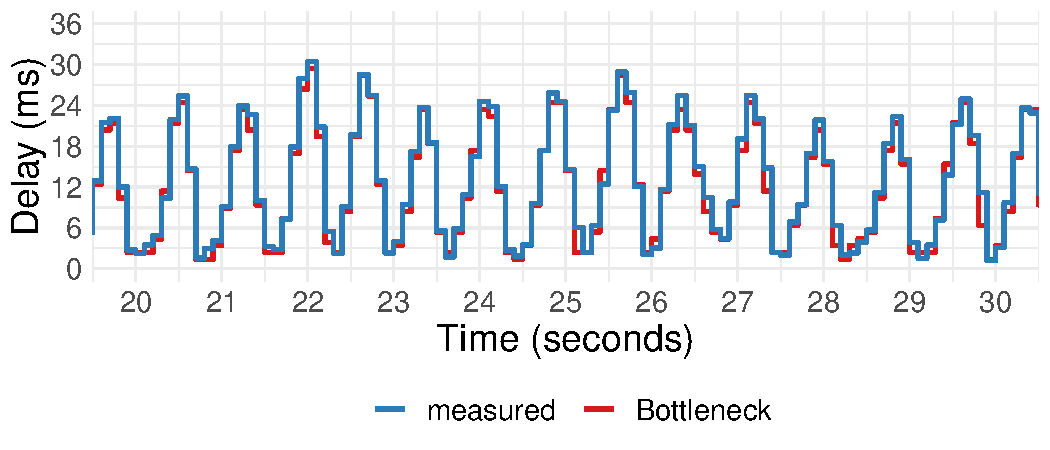
\includegraphics[width=\maxwidth]{figure/micro:time-delay-1} 

\end{knitrout}

    \caption{A representative example of the difference between \name's estimates and the actual values over a five second snapshot from one of the experiments in our evaluation. \name's estimates closely track the actual values over time, showing \name's ability to quickly observe changing network conditions. }
    \label{fig:micro:time-delay}
\end{figure}
